\question
Comando \verb|ping|.

\begin{parts}
  \part
  Comece a captura com o Wireshark e execute o comando 
  \verb|ping www.uol.com.br|. Observe os pacotes capturados com o 
  filtro para ICMP e identifique:

  \begin{subparts}
    \subpart
    O campo \emph{Protocol} no pacote IP.

    \begin{solution}
      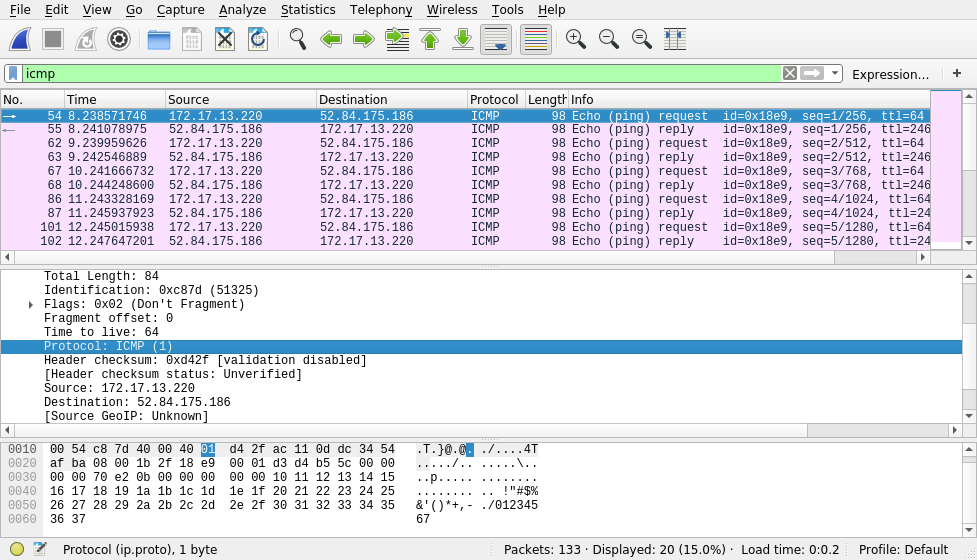
\includegraphics[width=\linewidth]{part-02/ex-1-1-1.png}
      \captionof{figure}{Campo \emph{Protocol} do pacote IP.}
      \vspace{1em}

      O campo \emph{Protocol} possui o valor \verb|ICMP (1)|. Este campo 
      mostra que a carga útil do pacote é o ICPM.
    \end{solution}

    \subpart
    Os tipos de mensagens ICMP trocados.

    \begin{solution}
      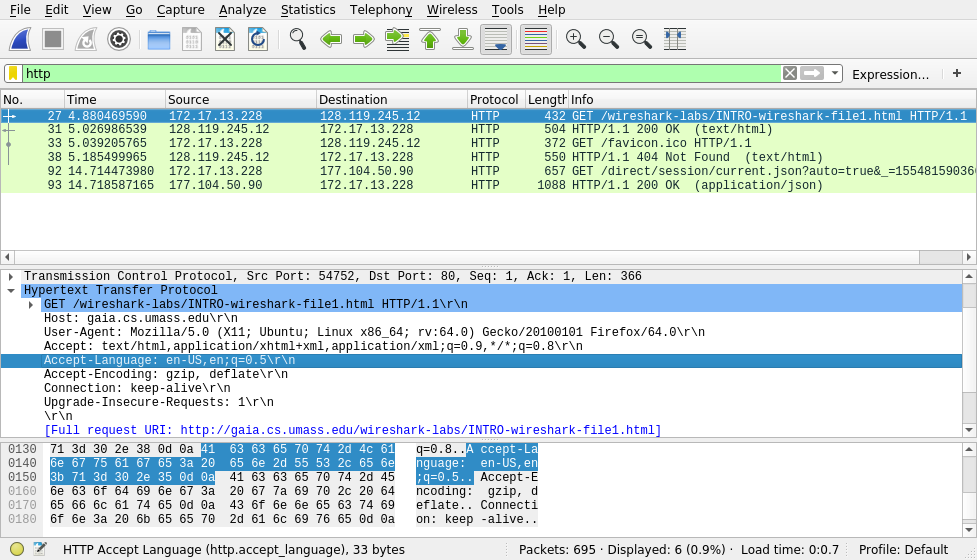
\includegraphics[width=\linewidth]{part-02/ex-1-1-2.png}
      \captionof{figure}{Dois tipos de mensagens.}
      \vspace{1em}

      O cliente envia um \verb|Echo (ping) request| e o servidor do UOL 
      responde com o \verb|Echo (ping) reply|.
    \end{solution}

    \subpart
    As demais informações que constam nos pacotes trocados.

    \begin{solution}
      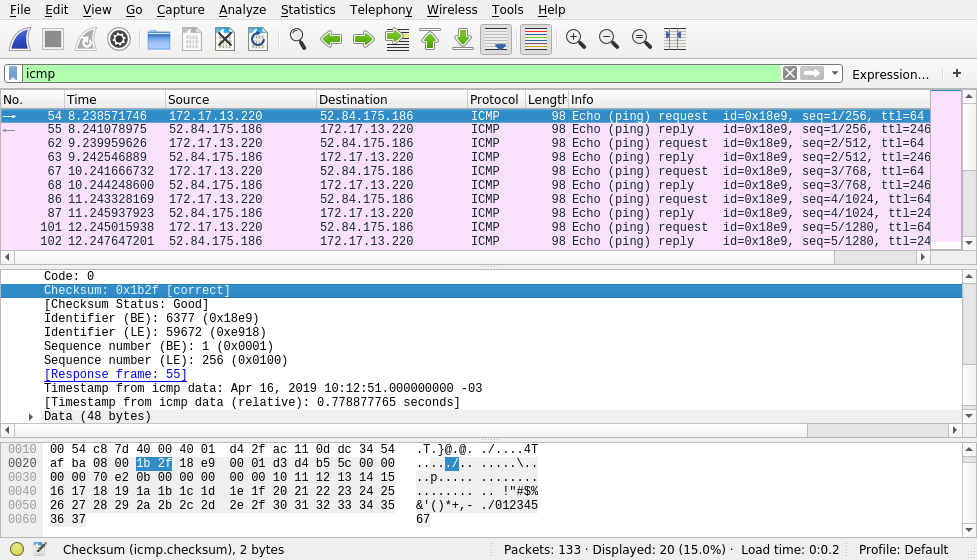
\includegraphics[width=\linewidth]{part-02/ex-1-1-3.png}
      \captionof{figure}{Informações nos pacotes trocados.}
      \vspace{1em}

      O pacote possui um \emph{checksum} e um \emph{identifier}, pois 
      podem ter vários processos de \verb|ping| na máquina e torna-se 
      necessário diferenciá-los para enviar a resposta para o destino 
      correto. O pacote também possui um \emph{sequence number}, que
      permite identificar se o pacote foi perdido.
    \end{solution}

    \subpart
    O tempo de ida e volta das mensagens ICMP. Compare com os tempos
    mostrados na saída do terminal.

    \begin{solution}
      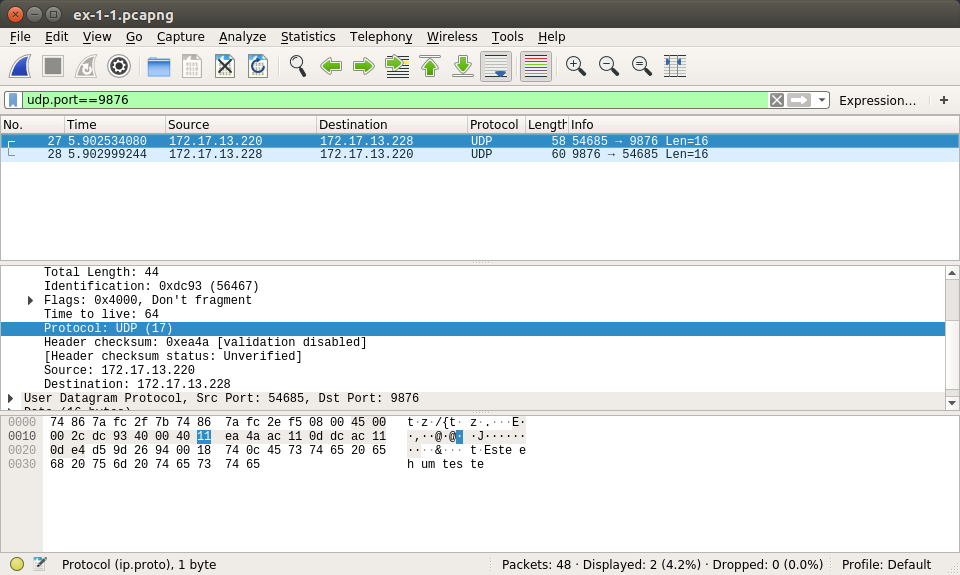
\includegraphics[width=\linewidth]{part-02/ex-1-1-4.png}
      \captionof{figure}{Tempos de ida e volta.}
      \vspace{1em}

      Os tempos de ida e volta tem uma média de \SI{3}{\milli\second}. 
      Em comparação coma saída no terminal, há uma pequena diferença de 
      \SI{0.01}{\milli\second}.
    \end{solution}
  \end{subparts}

  \pagebreak
  \part
  Repita o procedimento para o comando \verb|ping www.receita.fazenda.gov.br|.
  O que aconteceu? Explique.

  \begin{solution}
    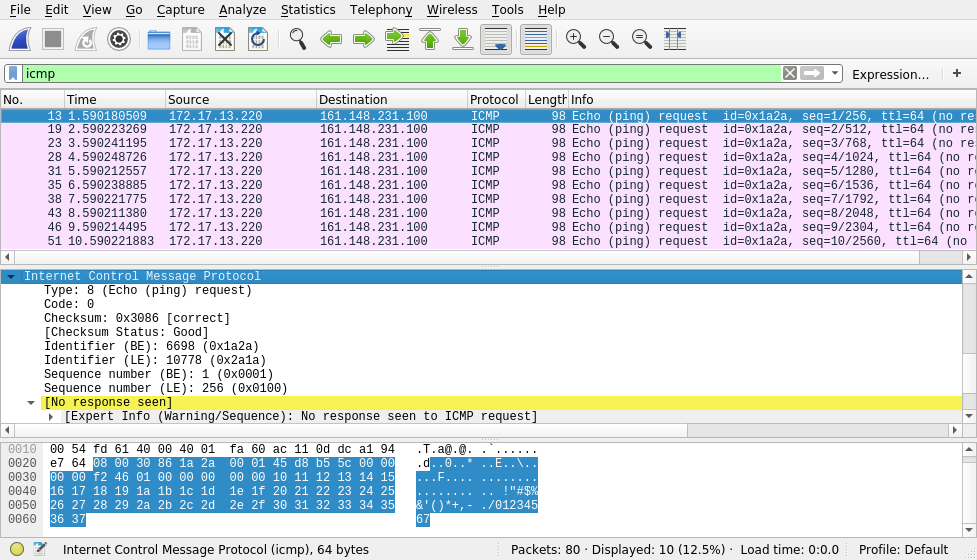
\includegraphics[width=\linewidth]{part-02/ex-1-2.png}
    \captionof{figure}{Pacotes enviados sem a resposta.}
    \vspace{1em}

    Houve perca total dos pacotes. Tal fato pode ser causado pelo site
    negar os acessos do \verb|ping|, filtrando-os e bloqueando-os.

    \begin{Verbatim}[label={\$ ping www.receita.fazenda.gov.br -c 5}]
    PING receita.fazenda.gov.br (161.148.231.100) 56(84) bytes of data.

    --- receita.fazenda.gov.br ping statistics ---
    5 packets transmitted, 0 received, 100% packet loss, time 4084ms
    \end{Verbatim}
  \end{solution}

  \part
  Comente sobre o tempo de resposta obtido com o \verb|ping| para:

  \begin{subparts}
    \subpart
    \verb|127.0.0.1|

    \begin{solution}
      Tempo de \SI{0.026}{\milli\second}. O \emph{localhost} é a 
      própria máquina, portanto a resposta é rápida.
    \end{solution}

    \subpart
    \verb|www.ufabc.edu.br|

    \begin{solution}
      Tempo de \SI{0.874}{\milli\second}. Estando dentro da rede da 
      UFABC, a resposta também é rápida.
    \end{solution}

    \subpart
    \verb|www.usp.br|

    \begin{solution}
      Tempo de \SI{2.54}{\milli\second}. A USP possui um sistema 
      autônomo mais distante, saindo do roteador da UFABC até 
      chegar ao da USP.
    \end{solution}

    \subpart
    \verb|www.google.com.br|

    \begin{solution}
      Tempo de \SI{2.90}{\milli\second}. Aproximadamente a mesma 
      distância para a USP, possuindo pontos de troca de tráfego.
    \end{solution}

    \pagebreak
    \subpart
    \verb|www.mit.edu|

    \begin{solution}
      Tempo de \SI{1.75}{\milli\second}. O site do MIT usa um serviço 
      de distribuição de conteúdo, assim a \emph{Akamai} faz uma cópia
      do site do MIT para uma localização mais próxima do cliente, em 
      São Paulo.
    \end{solution}

    \subpart
    \verb|www.ufl.edu|

    \begin{solution}
      Tempo de \SI{127}{\milli\second}. São Paulo possui uma ligação 
      de fibra óptica até Miami, então a latência para conectar aos 
      EUA é muito maior.
    \end{solution}

    \subpart
    \verb|www.cs.ubc.ca|

    \begin{solution}
      Tempo de \SI{181}{\milli\second}. A rota utilizada é mais longa, 
      logo aumenta-se o tempo.
    \end{solution}

    \subpart
    \verb|www.chat.ru|

    \begin{solution}
      Tempo de \SI{267}{\milli\second}. Utiliza-se uma rota pelos 
      EUA para chegar a Rússia, aumentando a ordem de grandeza.
    \end{solution}
  \end{subparts}
\end{parts}

\question
Comando \verb|traceroute|.

\begin{parts}
  \part
  Execute o comando \verb|traceroute www.uol.com.br|. Observe os pacotes
  capturados com o filtro para ICMP e identifique:

  \begin{subparts}
    \subpart
    O valor do TTL de cada mensagem enviada.

    \begin{solution}
      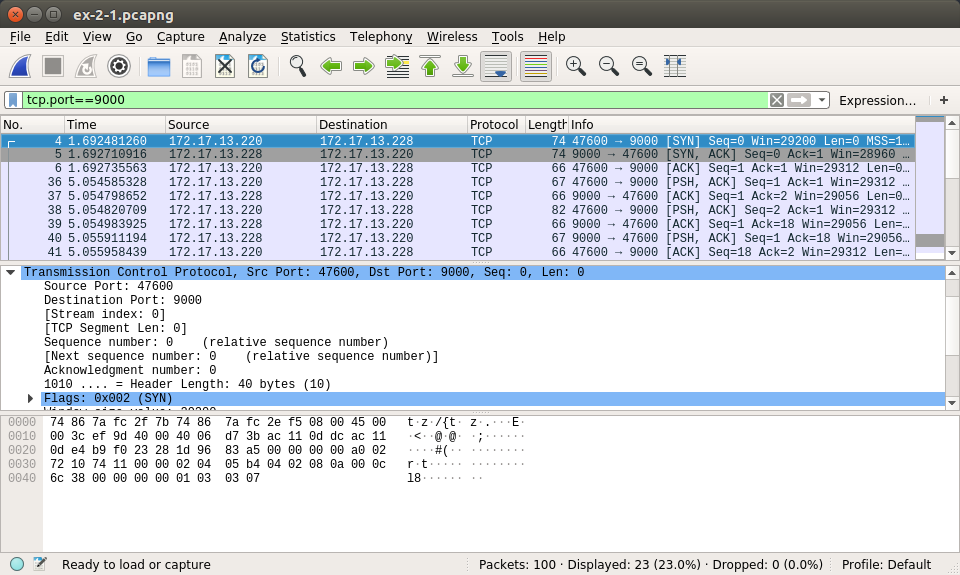
\includegraphics[width=\linewidth]{part-02/ex-2-1-1.png}
      \captionof{figure}{\emph{TTL} dos pacotes enviados.}
      \vspace{1em}

      O valor do TTL vai sendo incrementado em uma unidade a cada pacote.
    \end{solution}

    \pagebreak
    \subpart
    O tipo de mensagem ICMP recebida.

    \begin{solution}
      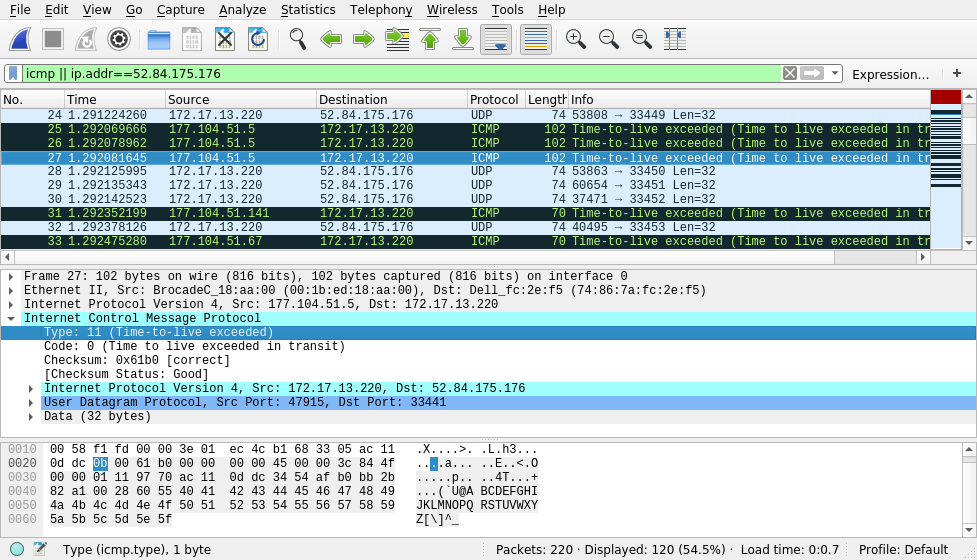
\includegraphics[width=\linewidth]{part-02/ex-2-1-2.png}
      \captionof{figure}{Mensagens ICMP recebidas.}
      \label{fig:2-1-2}
      \vspace{1em}

      O tipo utilizado é o \verb|11 (Time-to-live exceeded)|.
    \end{solution}

    \subpart
    As demais informações que constam nos pacotes trocados.

    \begin{solution}
      A mensagem possui um UDP encapsulado e o IP, como observa-se
      na Figura \ref{fig:2-1-2}.
    \end{solution}

    \subpart
    Quantas mensagens são enviadas e recebidas. Comente sobre a
    sequência de mensagens enviadas, explicando o funcionamento
    do comando.

    \begin{solution}
      Envia-se três mensagens e recebe-se três respostas. As mensagens
      são enviadas com o TTL aumentando de 1 em 1 e este TTL se expira
      com um hop maior, assim é possível identificar a rota.
    \end{solution}
  \end{subparts}

  \part
  Repita o comando \verb|traceroute| e comente sobre os resultados obtidos
  na saída para os seguintes endereços:

  \begin{subparts}
    \subpart
    \verb|127.0.0.1|

    \begin{solution}
      O localhost não possui roteadores intermediários, logo não há saída.
    \end{solution}

    \subpart
    \verb|www.ufabc.edu.br|

    \begin{solution}
      Para o site da UFABC só existe um roteador intermediário.

    \begin{Verbatim}[label={\$ traceroute www.ufabc.edu.br}, fontsize=\footnotesize]
    traceroute to www.ufabc.edu.br (177.104.50.120), 30 hops max, 60 byte packets
     1  172.17.13.193 (172.17.13.193)  0.237 ms  0.317 ms  0.364 ms
     2  177.104.51.29 (177.104.51.29)  8.442 ms  8.506 ms  8.607 ms
    \end{Verbatim}
    \end{solution}

    \subpart
    \verb|www.usp.br|

    \begin{solution}
      Sai-se do sistema autônomo da UFABC, passando pelo ponto de São Paulo,
      chegando no sistema autônomo da USP, através do ponto de troca de tráfego.

    \begin{Verbatim}[label={\$ traceroute www.usp.br}, fontsize=\footnotesize]
    traceroute to www.usp.br (200.144.248.41), 30 hops max, 60 byte packets
     1  172.17.13.193 (172.17.13.193)  1.627 ms  1.715 ms  1.746 ms
     2  177.104.51.29 (177.104.51.29)  0.285 ms  0.363 ms  0.396 ms
     3  177.104.51.5 (177.104.51.5)  0.998 ms  0.992 ms  0.974 ms
     4  177.104.51.141 (177.104.51.141)  1.619 ms  1.738 ms  1.827 ms
     5  177.104.51.67 (177.104.51.67)  5.348 ms  3.357 ms  6.729 ms
     6  as28571.saopaulo.sp.ix.br (187.16.216.20)  2.689 ms  2.505 ms  2.654 ms
     7  143.107.151.62 (143.107.151.62)  2.882 ms  2.404 ms  2.267 ms
     8  10.20.30.1 (10.20.30.1)  2.940 ms  3.026 ms  2.908 ms
    \end{Verbatim}
    \end{solution}

    \subpart
    \verb|www.google.com.br|

    \begin{solution}
      O Google também possui acordo com o ponto de troca de tráfego de 
      São Paulo.

    \begin{Verbatim}[label={\$ traceroute www.google.com.br}, fontsize=\footnotesize]
    traceroute to www.google.com.br (216.58.202.131), 30 hops max, 60 byte packets
     1  172.17.13.193 (172.17.13.193)  1.190 ms  1.369 ms  1.458 ms
     2  177.104.51.29 (177.104.51.29)  0.315 ms  0.361 ms  0.411 ms
     3  177.104.51.5 (177.104.51.5)  0.951 ms  0.940 ms  0.916 ms
     4  177.104.51.141 (177.104.51.141)  1.133 ms  1.233 ms  1.381 ms
     5  200.133.254.189 (200.133.254.189)  1.778 ms  1.842 ms  1.753 ms
     6  200.143.254.209 (200.143.254.209)  1.806 ms  1.810 ms  1.974 ms
     7  as15169.saopaulo.sp.ix.br (187.16.216.55)  2.780 ms as15169.saopaulo.sp.ix.br 
     (187.16.218.58)  2.787 ms      as15169.saopaulo.sp.ix.br (187.16.216.55)  2.502 ms
     8  108.170.245.161 (108.170.245.161)  3.130 ms  3.046 ms 108.170.245.129 
     (108.170.245.129)  3.166 ms
     9  72.14.239.227 (72.14.239.227)  3.197 ms  3.189 ms 72.14.239.225 (72.14.239.225)  
     2.924 ms
    10  gru06s29-in-f3.1e100.net (216.58.202.131)  2.785 ms  2.762 ms  3.127 ms
    \end{Verbatim}
    \end{solution}

    \subpart
    \verb|www.mit.edu|

    \begin{solution}
      Passa-se pelo sistema autonomo de SP, passando por mais hops.

    \begin{Verbatim}[label={\$ traceroute www.mit.edu}, fontsize=\footnotesize]
    traceroute to www.mit.edu (104.78.57.24), 30 hops max, 60 byte packets
     1  172.17.13.193 (172.17.13.193)  0.261 ms  0.297 ms  0.375 ms
     2  177.104.51.29 (177.104.51.29)  0.268 ms  0.394 ms  0.429 ms
     3  177.104.51.5 (177.104.51.5)  0.924 ms  0.907 ms  0.889 ms
     4  177.104.51.141 (177.104.51.141)  2.430 ms  2.138 ms  2.269 ms
     5  177.104.51.67 (177.104.51.67)  2.764 ms  3.132 ms  3.440 ms
     6  as20940.saopaulo.sp.ix.br (187.16.220.8)  5.186 ms  3.723 ms  4.799 ms
    \end{Verbatim}
    \end{solution}

    \subpart
    \verb|www.ufl.edu|

    \begin{solution}
      Utilizou-se o \emph{link} normal no lugar do acadêmico.

    \begin{Verbatim}[label={\$ traceroute www.ufl.edu}, fontsize=\footnotesize]
    traceroute to www.ufl.edu (128.227.9.98), 30 hops max, 60 byte packets
     1  172.17.13.193 (172.17.13.193)  7.262 ms  7.363 ms  7.426 ms
     2  177.104.51.29 (177.104.51.29)  5.923 ms  5.981 ms  6.056 ms
     3  177.104.51.5 (177.104.51.5)  0.894 ms  0.902 ms  0.889 ms
     4  177.104.51.141 (177.104.51.141)  1.237 ms  1.397 ms  1.074 ms
     5  200.133.254.189 (200.133.254.189)  1.730 ms  1.703 ms  1.819 ms
     6  200.143.254.209 (200.143.254.209)  2.280 ms  1.781 ms  1.769 ms
     7  170.79.213.7 (170.79.213.7)  107.116 ms  107.181 ms  107.109 ms
    [...]
    18  ufl.edu (128.227.9.98)  127.541 ms  127.456 ms  127.728 ms
    \end{Verbatim}
    \end{solution}

    \subpart
    \verb|www.cs.ubc.ca|

    \begin{solution}
      Também se utilizou o \emph{link} normal.

    \begin{Verbatim}[label={\$ traceroute www.cs.ubc.ca}, fontsize=\footnotesize]
    traceroute to www.cs.ubc.ca (142.103.6.5), 30 hops max, 60 byte packets
     1  172.17.13.193 (172.17.13.193)  5.197 ms  5.255 ms  5.320 ms
     2  177.104.51.29 (177.104.51.29)  4.992 ms  5.089 ms  5.080 ms
     3  177.104.51.5 (177.104.51.5)  1.017 ms  1.006 ms  0.979 ms
     4  177.104.51.141 (177.104.51.141)  1.405 ms  1.156 ms  1.284 ms
     5  177.104.51.67 (177.104.51.67)  3.434 ms  3.680 ms  3.974 ms
    [...]
    14  137.82.88.122 (137.82.88.122)  223.014 ms  207.746 ms  207.704 ms
    15  a1-a0.net.ubc.ca (142.103.78.249)  237.604 ms  224.392 ms *
    \end{Verbatim}
    \end{solution}

    \subpart
    \verb|www.chat.ru|

    \begin{solution}
      Passa-se pelo acordo de troca de tráfego, passando pela internet
      comercial e não pelo \emph{link} acadêmico.

    \begin{Verbatim}[label={\$ traceroute www.cs.ubc.ca}, fontsize=\footnotesize]
    traceroute to www.chat.ru (77.244.218.84), 30 hops max, 60 byte packets
     1  172.17.13.193 (172.17.13.193)  0.253 ms  1.861 ms  1.854 ms
     2  177.104.51.29 (177.104.51.29)  1.844 ms  0.402 ms  0.461 ms
     3  177.104.51.5 (177.104.51.5)  0.985 ms  0.973 ms  0.951 ms
     4  177.104.51.141 (177.104.51.141)  1.464 ms  1.160 ms  1.311 ms
     5  200.133.254.189 (200.133.254.189)  1.784 ms  1.778 ms  1.795 ms
     6  200.143.254.209 (200.143.254.209)  2.504 ms  2.137 ms  3.728 ms
     7  170.79.213.7 (170.79.213.7)  107.510 ms  107.500 ms  107.489 ms
     8  206.41.108.23 (206.41.108.23)  107.466 ms nota.he.net (198.32.124.176)
    [...]
    21  * 57.msk.net.selectel.ru (188.93.17.57)  262.191 ms *
    \end{Verbatim}
    \end{solution}
  \end{subparts}
\end{parts}

\question
Comando \verb|arp|.

\begin{parts}
  \part
  Use o comando \verb|arp -e| na linha de comando para listar o conteúdo da
  \emph{cache} ARP. Verifique quais são os endereços que estão na \emph{cache}.

  \begin{solution}
    O \emph{cache} possui alguns endereços da rede local da UFABC.

    \begin{Verbatim}[label={\$ arp -e}]
    Endereço TipoHW EndereçoHW Flags Máscara Iface
    172.17.13.194   ether   00:1b:ed:16:16:00   C   eno1
    172.17.13.195   ether   00:1b:ed:18:aa:00   C   eno1
    172.17.13.193   ether   02:e0:52:a8:f6:01   C   eno1
    \end{Verbatim}
  \end{solution}

  \pagebreak
  \part
  Inicie a captura com o Wireshark e execute o comando \verb|ping| para um
  computador da rede local ainda não acessado e depois verifique novamente
  a tabela ARP (ex.: \verb|ping 172.17.13.247|). Verifique também os pacotes
  ARP capturados. Veja os campos de cabeçalho, observando a requisição
  e a resposta. Verifique quais são os endereços MAC. Comente sobre
  o funcionamento do protocolo.

  \begin{solution}
    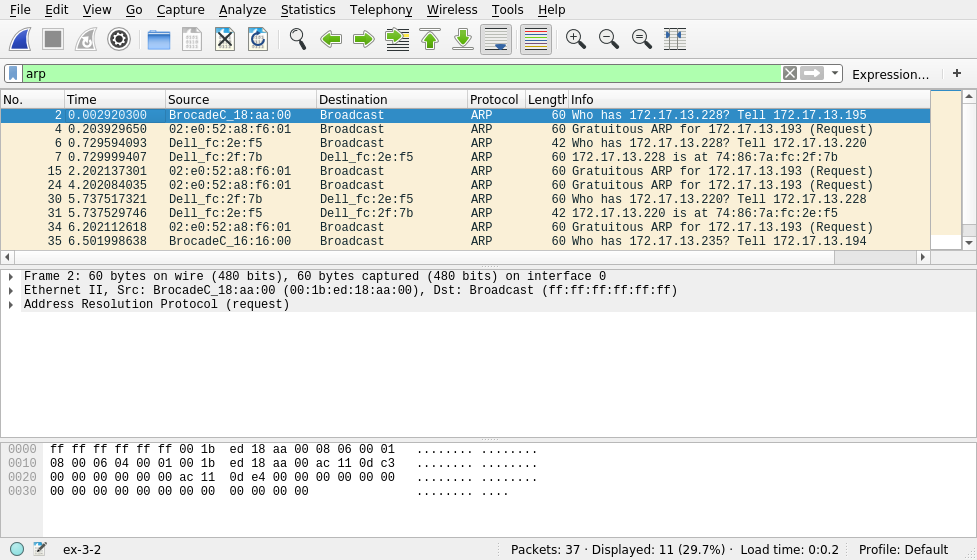
\includegraphics[width=\linewidth]{part-02/ex-3-2.png}
    \captionof{figure}{Pacotes do tipo ARP capturados.}
    \vspace{1em}

    Transmite-se via \emph{broadcast} uma requisição de tradução do IP 
    especificado, informando o MAC e IP da máquina. A máquina que possui 
    este endereço MAC, se identifica e retorna o IP e MAC desejado. 
    O endereço MAC da máquina origem é \verb|74:86:7a:fc:2e:f5| e o 
    de destino é \verb|74:86:7a:fc:2f:7b|.
  \end{solution}

  \pagebreak
  \part
  Execute novamente o comando \verb|ping| para a mesma máquina do item 3.2.
  Foram capturados pacotes ARP? Justifique.

  \begin{solution}
    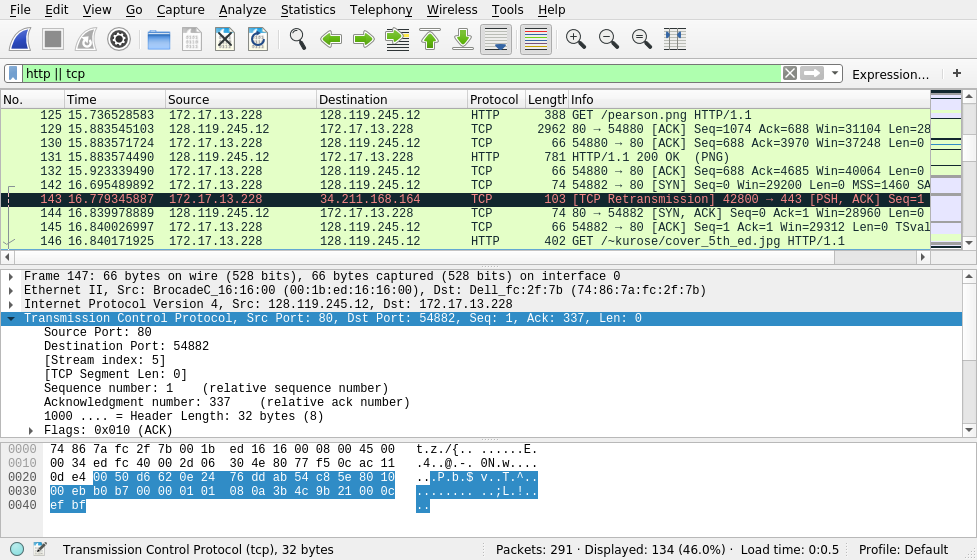
\includegraphics[width=\linewidth]{part-02/ex-3-3.png}
    \captionof{figure}{Efetua-se diretamente o \texttt{ping}.}
    \vspace{1em}

    Não foram capturados pacotes ARP pois o endereço MAC já fica em
    \emph{cache}, assim não é necessário realizar uma nova requisição
    enquanto ainda for válido.
  \end{solution}

  \part
  Remova as entradas da tabela ARP com o comando \verb|arp -d IP|, em que
  \verb|IP| é o endereço IP do \emph{host} a ser removido, e liste o conteúdo
  da \emph{cache}. O que aconteceu? Em seguida, execute o comando 
  \verb|ping IP|. Agora os pacotes ARP foram capturados? Justifique.

  \begin{solution}
    Sim, agora novos pacotes ARP foram capturados já que não existe no
    \emph{cache} o endereço que foi removido anteriormente.

    \begin{Verbatim}[label={\$ arp -e}]
    Endereço TipoHW EndereçoHW Flags Máscara Iface
    172.17.13.194   ether   00:1b:ed:16:16:00   C   eno1
    172.17.13.195   ether   00:1b:ed:18:aa:00   C   eno1
    172.17.13.193   ether   02:e0:52:a8:f6:01   C   eno1
    172.17.13.228   (incompleto)                    eno1
    \end{Verbatim}
  \end{solution}
  
\end{parts}

\question
Comando \verb|dhclient|.

\begin{parts}
  \part
  No Ubuntu, pare o \emph{Network Manager} com o comando 
  \verb|sudo service network-manager stop|. Libere o endereço IP, 
  executando o comando \verb|sudo dhclient -r eth0|. Execute 
  \verb|ifconfig| para verificar o seu endereço IP. O seu computador
  ainda tem endereço IP? Tente acessar qualquer coisa na rede 
  (o UOL, por exemplo).

  \begin{solution}
    O computador não possui mais endereço IP, logo não é possível acessar
    qualquer coisa na rede. Necessitou-se executar os comandos
    \verb|ifconfig eno1 down| para liberar o IP.

    \begin{Verbatim}[label={\$ ifconfig}]
    lo        Link encap:Loopback Local  
              inet end.: 127.0.0.1  Masc:255.0.0.0
              endereço inet6: ::1/128 Escopo:Máquina
              UP LOOPBACK RUNNING  MTU:65536  Métrica:1
              pacotes RX:1955 erros:0 descartados:0 excesso:0 quadro:0
              Pacotes TX:1955 erros:0 descartados:0 excesso:0 portadora:0
              colisões:0 txqueuelen:1 
              RX bytes:315420 (315.4 KB) TX bytes:315420 (315.4 KB)
    \end{Verbatim}
  \end{solution}

  \part
  Inicie a captura com o Wireshark e execute o comando 
  \verb|sudo dhclient eth0| para obter novas configurações de rede 
  (incluindo o endereço IP). Execute novamente o comando \verb|ifconfig|
  e tente acessar a rede. Funcionou?

  \begin{solution}
    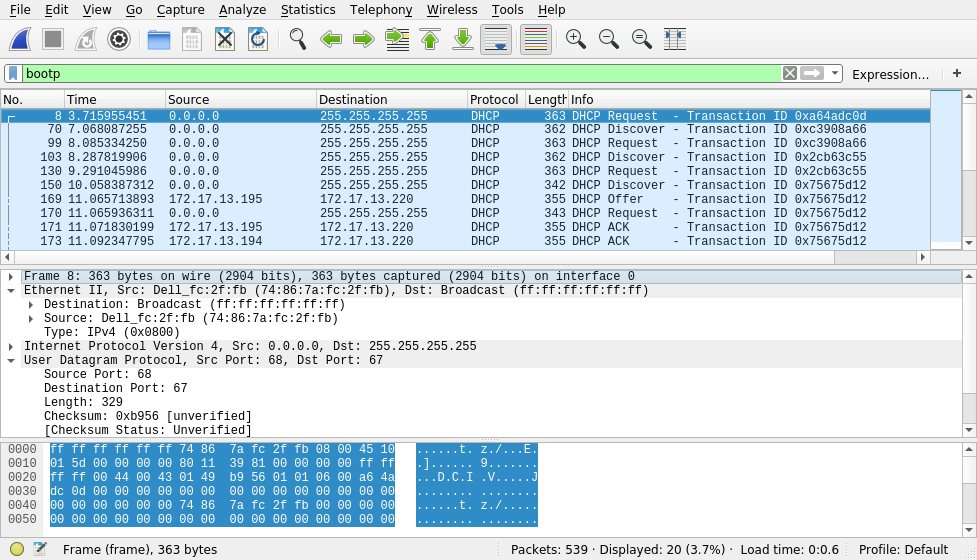
\includegraphics[width=\linewidth]{part-02/ex-4-2.png}
    \captionof{figure}{Pacotes do protocolo DHCP capturados.}
    \label{fig:4-2}
    \vspace{1em}

    Agora a máquina obteve um novo endereço IP e é capaz de acessar a rede.
  \end{solution}

  \part
  Comente sobre as informações que estão presentes nos pacotes DHCP
  capturados (use o filtro ``bootp'' no Wireshark), explicando como
  funciona o protocolo.

  \begin{solution}
    Há uma conversação no protocolo através do DHCP Discover, Offer,
    Request e ACK. O cliente requisita os parâmetros e o servidor DHCP
    confirma através do ACK que os parâmetros estão corretos. A troca
    dos pacotes pode ser observada na Figura \ref{fig:4-2}.
  \end{solution}
\end{parts}

\question
Comando \verb|route|.

\begin{parts}
  \part
  Use o comando \verb|route| para observar a tabela de roteamento do seu
  computador. Que rotas estão presentes?

  \begin{solution}
    Visualiza-se o roteador entregue pelo DHCP.

    \begin{Verbatim}[label={\$ route}, fontsize=\small]
    Tabela de Roteamento IP do Kernel
    Destino         Roteador        MáscaraGen.    Opções Métrica Ref   Uso Iface
    default         172.17.13.193   0.0.0.0         UG    0      0        0 eno1
    172.17.13.192   *               255.255.255.192 U     0      0        0 eno1   
    \end{Verbatim}
  \end{solution}

  \part
  Exclua a rota padrão (\emph{default}) da tabela de roteamento, com o
  comando \texttt{sudo route del default}. Tente acessar um servidor fora
  da sua sub-rede local, como o UOL. Ocorreu algum problema? Justifique.

  \begin{solution}
    Não é possível acessar pois a rede deixou de funcionar, não é possível
    alcançar outras sub-redes já que não há como realizar a rota da máquina
    atual para uma exterior.
  \end{solution}

  \part
  Execute o comando \verb|ping| para o servidor do item 5.2, de preferência
  para o seu endereço IP. Qual foi a mensagem de erro?

  \begin{solution}
    Não há mensagem de erro pois uma rota dentro de uma sub-rede local
    ainda continua funcionando.

    \begin{Verbatim}[label={\$ ping 172.17.13.193 -c 3}]
    PING 172.17.13.193 (172.17.13.193) 56(84) bytes of data.
    64 bytes from 172.17.13.193: icmp_seq=1 ttl=64 time=5.66 ms
    64 bytes from 172.17.13.193: icmp_seq=2 ttl=64 time=6.69 ms
    64 bytes from 172.17.13.193: icmp_seq=3 ttl=64 time=7.61 ms
    
    --- 172.17.13.193 ping statistics ---
    3 packets transmitted, 3 received, 0% packet loss, time 2001ms
    rtt min/avg/max/mdev = 5.664/6.656/7.612/0.798 ms
    \end{Verbatim}
  \end{solution}

  \part
  Execute um comando \verb|ping| para uma máquina da sua sub-rede local.
  Esse comando foi executado? Justifique.

  \begin{solution}
    O comando foi executado pois uma rota dentro de uma sub-rede local
    ainda continua funcionando mesmo após da remoção, já que o roteamento
    inverso do \emph{switch} ainda continua funcionando.

    \begin{Verbatim}[label={\$ ping 172.17.13.228 -c 3}]
    PING 172.17.13.228 (172.17.13.228) 56(84) bytes of data.
    64 bytes from 172.17.13.228: icmp_seq=1 ttl=64 time=0.215 ms
    64 bytes from 172.17.13.228: icmp_seq=2 ttl=64 time=0.229 ms
    64 bytes from 172.17.13.228: icmp_seq=3 ttl=64 time=0.231 ms
    
    --- 172.17.13.228 ping statistics ---
    3 packets transmitted, 3 received, 0% packet loss, time 1998ms
    rtt min/avg/max/mdev = 0.215/0.225/0.231/0.007 ms
    \end{Verbatim}
  \end{solution}

  \part
  Adicione novamente a rota padrão, com o comando 
  \verb|sudo route add default gw IP|, em que \verb|IP| é o endereço 
  do roteador padrão exibido no item 5.1. Repita o \verb|ping| para 
  o servidor externo. Funcionou? Justifique.

  \begin{solution}
    Reestabelece-se a rota, possibilitando com que consiga alcançar
    máquinas fora da rede local através do roteador.

    \begin{Verbatim}[label={\$ ping www.uol.com.br -c 5}, fontsize=\small]
    PING dftex7xfha8fh.cloudfront.net (52.84.175.186) 56(84) bytes of data.
    64 bytes from server-52-84-175-186.gru50.r.cloudfront.net (52.84.175.186): 
    icmp_seq=1 ttl=246 time=2.58 ms
    64 bytes from server-52-84-175-186.gru50.r.cloudfront.net (52.84.175.186): 
    icmp_seq=2 ttl=246 time=2.67 ms
    64 bytes from server-52-84-175-186.gru50.r.cloudfront.net (52.84.175.186): 
    icmp_seq=3 ttl=246 time=2.50 ms
    64 bytes from server-52-84-175-186.gru50.r.cloudfront.net (52.84.175.186): 
    icmp_seq=4 ttl=246 time=2.77 ms
    64 bytes from server-52-84-175-186.gru50.r.cloudfront.net (52.84.175.186): 
    icmp_seq=5 ttl=246 time=2.76 ms
    
    --- dftex7xfha8fh.cloudfront.net ping statistics ---
    5 packets transmitted, 5 received, 0% packet loss, time 4006ms
    rtt min/avg/max/mdev = 2.501/2.659/2.775/0.105 ms
    \end{Verbatim}
  \end{solution}
\end{parts}